\documentclass[12pt,a4paper]{article}
\usepackage[utf8]{inputenc}
\usepackage[ngerman]{babel}
\usepackage[T1]{fontenc}
\usepackage{amsmath}
\usepackage{amsfonts}
\usepackage{amssymb}
\usepackage{graphicx}
\usepackage{subfigure}
\author{Alexander Binsmaier, Manuel Mende, Yaroslav Direy}
\title{Evaluation des genetischen Algorithmus}
\begin{document}
\maketitle
\tableofcontents

\section{Multipopulationsalgorithmus}
Multipopulations-Algorithmen erlauben das parallele Entwickeln von Populationen. Sie können auf verschiedene Ziele ausgerichtet sein. Ein Austausch der Individuen zwischen Populationen soll zu einer Erhöhung der Diversität führen.
Bedingt durch die Notwendigkeit, Populationen als Gesamtheit behandeln und vor allem vermischen zu können, war es notwendig, die zuvor verwendete Implementierung des genetischen Algorithmus anzupassen. 

\subsection{Populationsbehandlung}
Die Verwaltung einer Population wurde in einer Klasse \emph{Population} gekapselt. Sie übernimmt die Erweiterung der Population um neue Chromosome, sowie die Reduktion auf die vorgegeben Populationsgrößen. Auch die Initialisierung der Chromosome wird von der Populationsklasse übernommen. Die Reduktion der Chromosomen-Anzahl erfolgt durch aussortieren der \glqq schwächsten\grqq Individuen. Sie zeichnen sich durch die schlechteste Fitness innerhalb der Population aus.

\subsection{Genetischer Algorithmus}
Die erste Version des genetischen Algorithmus verfügte lediglich über eine Hauptroutine, die die zyklische Evolution der Chromosome vornahm. Um mehrere Algorithmen verwenden und eine Interaktion gewährleisten zu können, musste eine schrittweise Umsetzung der Evolution integriert werden. Aus Gründen der Übersichtlichkeit und Wartbarkeit wurde eine neue Klasse \textsf{GenericGA} angelegt. Diese weist zwei Vorteile gegenüber der ersten Implementierung auf. Die Algorithmus-Klasse ist lediglich für die Umsetzung der genetischen Operationen zuständig, sämtliche die Population betreffenden Operationen wie Initialisierung und Reduktion werden in der Populations-Klasse behandelt. Zudem kann die Evolution Schrittweise von einer übergeordneten Kontrollinstanz durchgeführt werden. Damit ergibt sich die Flexibilität, verschiedene Instanzen zu erzeugen, die Populationen zu mischen, und erneut einige Iterationen zu durchlaufen. \\
Die schrittweise Evolution wird durch die Funktion \begin{quote}
\textsf{runEpoch(population)}
\end{quote} gewährleistet. Sie modifiziert Chromosome der übergebenen Population. Dazu werden die Funktionen-Handles der \textsf{GenericGA}-Instanz verwendet, die durch den Konstruktor gesetzt werden müssen. Als problematisch erweist sich die Ermittlung der neuen Fitness-Werte. An sich ist es Sinnvoll, vor jedem Selektionsprozess die Fitnessfunktionen zu berechnen. Damit wäre für einen nächsten Durchlauf die alte Fitness für die Rekombination verfügbar. Leider kann das im Falle von Migrationen zu Problemen führen, da hier Chromosome aus anderen Populationen übernommen werden. Weil die verschiedenen Populationen durch unterschiedliche Fitnessfunktionen geprägt werden, ist nach einer Migration vor einer erneuten Rekombination eine erneute Fitnessberechnung durchzuführen. Die Schnittstelle \textsf{runEpoch} setzt deshalb Populationen mit validen Fitnessinformationen voraus. Dazu kann die Funktion \begin{quote}
\textsf{computeFitness(population)} \end{quote} einer \textsf{GenericGA}-Instanz verwendet werden. Sie weißt jedem Chromosom die durch die Fitnessfunktion des genetischen Algorithmus bedingte Fitness zu. Sollen mehrere Evolutionsepochen ohne Migration durchlaufen werden, kann die Schnittstelle 
\begin{quote}
\textsf{runEpochs(population, iterations)}
\end{quote} verwendet werden. Sie setzt keine validen Fitness-Informationen voraus.

\subsection{Kontrollinstanz}
Die Kontrollinstanz koordiniert die Ausführung der einzelnen genetischen Algorithmen. Die Initialisierung erfolgt lediglich mit der vorgesehenen Größe der Population. Die Klasse \textsf{MultiPopulationGA} enthält die Funktionen
\begin{quote}
\textsf{addPopulation(fitness\_handle)} sowie \\
\textsf{runMPGA(migrations\_rate, epochs\_between\_migrations, migration\_cycles, policy)}
\end{quote}
Erstere dient dem konfigurieren der genetischen Algorithmen -- hier kann eine besondere Fitnessfunktion übergeben werden -- die zweite Funktion dient der Evolution der Populationen. Die Abarbeitung kann durch die Parameter eingestellt werden. Die Migrationsrate entspricht der Anzahl der Chromosome, die in jeder Population getauscht werden sollen. Zudem kann die Anzahl Epochen zwischen Migrationsvorgängen und die Anzahl an Migrationsvorgängen festgelegt werden. Der Parameter \textsf{policy} dient dem Wechsel zwischen Ring-, Nachbar- und uneingeschränkter Migration.

\section{Ausgewählte Testfälle}
Zur Definition der einzelnen Populationen für den genetischen Algorithmus wurden Äquivalenzklassen der Testfälle analytisch hergeleitet.
\subsection{Gruppierung}
Die Anzahl der Äquivalenzklassen für die gesuchten Testfälle wird durch Kombination von Fahrzeugposition im Verhältnis zur Parklücke (left/right) sowie von Fahrzeugausrichtung (up/down/left/right) bestimmt. Somit ergeben sich acht Gruppen der gesuchten Testfälle.
\subsection{Dedizierte Fitnessfunktionen}
Für jede Äquivalenzklasse wurde eine Fitnessfunktion so definiert, dass die Testfälle mit gesuchten Eigenschaften innerhalb einer Population eine höhere Wertung erhalten. Somit wird der Selektionsdruck vom genetischen Algorithmus in eine für gegebenen Population gewünschte Richtung geleitet. Die Testfälle, die von den gewünschten Eigenschaften stark abweichen werden dagegen mit einem schlechten Wert der Fitnessfunktion bestraft und folglich aussortiert.
\section{Bewertung}
Die Ergebnisse vom genetischen Algorithmus mit mehreren Populationen weisen eine hohe Heterogenität im Vergleich zu einem einfachen genetischen Ansatz. Für jede Population wird der Selektionsdruck und somit auch die Konvergenz der gesuchten Testfälle mittels angepassten Fitnessfunktionen gesteuert.
\begin{figure}\centering
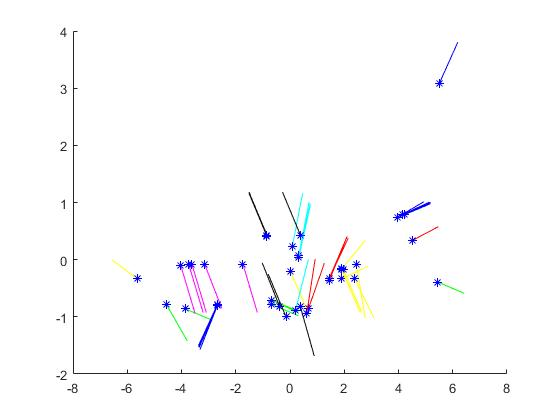
\includegraphics[width=.6\textwidth]{mpga_nomigration.jpg}
\caption{Visualisierung der Testfälle: MPGA ohne Migration}
\label{fig:mpganomig}
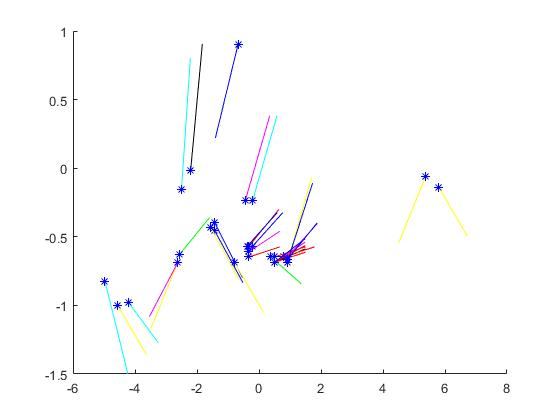
\includegraphics[width=.6\textwidth]{mpga_ring.jpg}
\caption{Visualisierung der Testfälle: MPGA Ring Migration}
\label{fig:mpgaring}
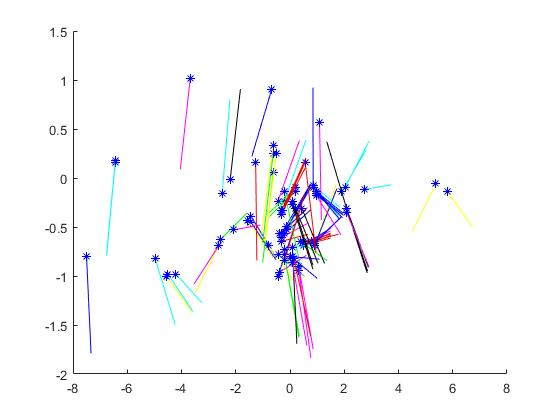
\includegraphics[width=.6\textwidth]{mpga_unrestricted.jpg}
\caption{Visualisierung der Testfälle: MPGA Unrestricted Migration}
\label{fig:mpgaunrest}

\end{figure}



\subsection{Eignung der Fitness-Funktionen}
Die Ergebnisse vom genetischen Algorithmus für acht  Populationen zeigen, dass die jeweiligen Fitnessfunktionen die Evolution der Testfälle in die gewünschte Richtung treiben. 
\subsection{Konvergenz der Populationen}
Die Konvergenz der Testfälle in der Populationen wird durch die verwendete Fitnessfunktion gesteuert. Durch eine hohe Bewertung der Testfälle mit gewünschten vorprogrammierten Eigenschaften bzw. durch Abwertung der unpassenden Testfälle konvergieren die Chromosome mit steigender Anzahl der Epochen zunehmend.
\subsection{Einfluss der Migrationen}
Für die Migration der Chromosome zwischen den Populationen wurden die 'ring', 'unrestricted' sowie die 'neighbour' Methode verwendet. Wie aus dem Vergleich der Ergebnisse ohne Migration ersichtlich hat Einsatz der genannten Migrationsmethoden positiv zur Erhöhung der Heterogenität der Testfälle innerhalb der Populationen beigetragen.
\begin{figure}\centering
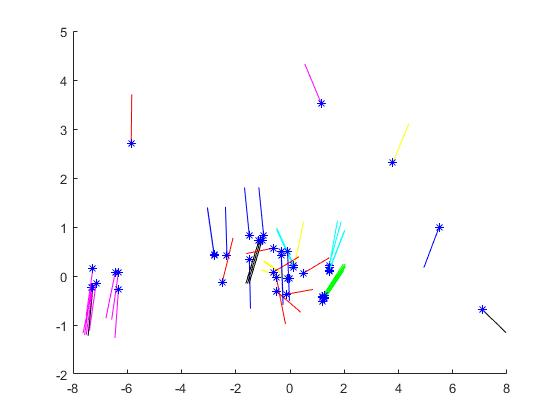
\includegraphics[width=.6\textwidth]{mpga_neighbour.jpg}
\caption{Visualisierung der Testfälle: MPGA Neighbour Migration}
\end{figure}
\label{fig:mpganeihb}
\end{document}
